\chapter{Quantum-Resistant Cryptographic Solutions}\label{chap:quantum_resistant}

\section{Post-Quantum Cryptography Overview}
Post-quantum cryptography (PQC) focuses on developing algorithms that remain secure against both classical and quantum computer attacks \parencite{bernstein2017post}. Unlike current public-key systems, these next-generation approaches rely on mathematical problems believed to remain hard even for quantum computers.

\section{Lattice-Based Cryptography}\label{sec:lattice}

\subsection{Mathematical Foundations}\label{subsec:lattice_math}
Lattice-based cryptography relies on hard problems in lattice theory:

\begin{equation}\label{eq:lattice}
    L(\mathbf{B}) = \{\mathbf{Bx} : \mathbf{x} \in \mathbb{Z}^n\}
\end{equation}

where $\mathbf{B}$ is the basis matrix.

\subsection{Learning With Errors (LWE)}\label{subsec:lwe}
The LWE problem forms the basis for many quantum-resistant schemes:

\begin{equation}\label{eq:lwe}
    \mathbf{b} = \mathbf{As} + \mathbf{e} \mod q
\end{equation}

where:
\begin{itemize}
    \item $\mathbf{A}$ is a random matrix
    \item $\mathbf{s}$ is the secret vector
    \item $\mathbf{e}$ is a small error vector
\end{itemize}

\begin{itemize}
    \item \textbf{Learning With Errors (LWE):} Forms the foundation for many lattice-based systems
    \item \textbf{NTRU:} One of the earliest and most studied lattice-based systems
    \item \textbf{CRYSTALS-Kyber:} Recently selected by NIST as a standard for key encapsulation
\end{itemize}

%\begin{figure}[h]
%    \centering
%    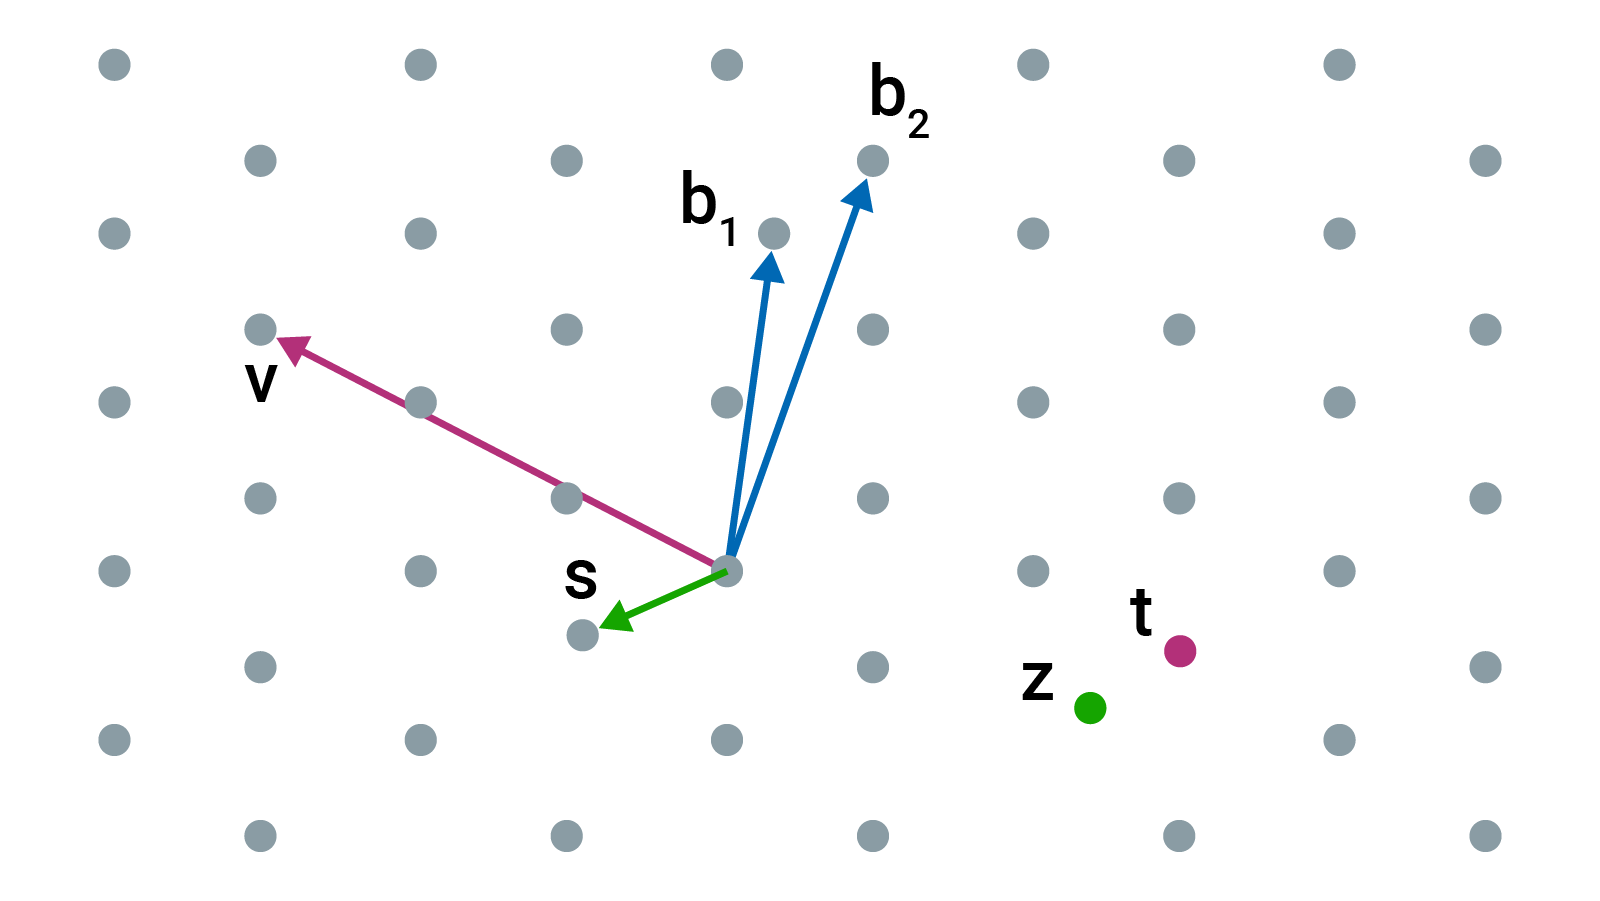
\includegraphics[width=0.7\textwidth]{lattice_cryptography.png}
%    \caption{Basic Concept of Lattice Cryptography}
%    \label{fig:lattice-crypto}
%\end{figure}

\section{Hash-Based Signatures}\label{sec:hash_based}

\subsection{Merkle Signatures}\label{subsec:merkle}
Construction of a Merkle tree:

% Commenting out missing image since merkle_tree.png is not available
%\begin{figure}[h]
%    \centering
%    \includegraphics[width=0.7\textwidth]{merkle_tree}
%    \caption{Merkle tree structure for hash-based signatures}
%    \label{fig:merkle_tree}
%\end{figure}

\subsection{SPHINCS+}\label{subsec:sphincs}
Key features of SPHINCS+:

\begin{itemize}
    \item \textbf{Security Properties:}
    \begin{itemize}
        \item Stateless design
        \item Hash-based security
        \item Forward security
    \end{itemize}
    \item \textbf{Performance Characteristics:}
    \begin{itemize}
        \item Signature size
        \item Verification speed
        \item Key generation time
    \end{itemize}
\end{itemize}

Hash-based signatures offer quantum resistance by relying solely on the security of cryptographic hash functions \parencite{bernstein2017post}. These functions are generally considered less vulnerable to quantum attacks compared to the mathematical problems underpinning traditional public-key cryptography.

\begin{itemize}
    \item \textbf{Merkle Signature Scheme:} A foundational approach using binary hash trees
    \item \textbf{SPHINCS+:} A modern, stateless hash-based signature scheme chosen by NIST
\end{itemize}

While hash-based signatures offer strong security guarantees, they typically produce larger signatures compared to traditional algorithms.

\section{Code-Based Cryptography}\label{sec:code_based}

\subsection{McEliece Cryptosystem}\label{subsec:mceliece}
The system uses error-correcting codes:

\begin{equation}\label{eq:mceliece}
    \mathbf{c} = \mathbf{mG'} + \mathbf{e}
\end{equation}

where:
\begin{itemize}
    \item $\mathbf{G'}$ is the public generator matrix
    \item $\mathbf{m}$ is the message
    \item $\mathbf{e}$ is the error vector
\end{itemize}

Code-based cryptography derives its security from the challenge of decoding general linear codes \parencite{bernstein2017post}. The McEliece system, proposed in 1978, exemplifies this approach's longevity and continued relevance in post-quantum cryptography.

\begin{itemize}
    \item \textbf{McEliece:} Has withstood decades of cryptanalysis
    \item Based on the computational difficulty of decoding linear codes
\end{itemize}

A notable characteristic of code-based systems is their requirement for larger key sizes, which can impact practical implementations.

\section{Multivariate Cryptography}\label{sec:multivariate}

\subsection{Rainbow Signature Scheme}\label{subsec:rainbow}
The multivariate quadratic system:

\begin{equation}\label{eq:rainbow}
    \mathbf{y} = \mathbf{F}(\mathbf{x}) = (f_1(\mathbf{x}), \ldots, f_m(\mathbf{x}))
\end{equation}

where each $f_i$ is a quadratic polynomial.

Multivariate cryptography is based on the difficulty of solving systems of multivariate polynomial equations:

\begin{itemize}
    \item Efficient for signatures but less practical for encryption
    \item Vulnerable to specific attacks in some implementations
\end{itemize}

\section{NIST Standardization Process}
NIST initiated its post-quantum cryptography standardization process in 2016 \parencite{alagic2020status}. After rigorous evaluation, several algorithms were selected:

\begin{itemize}
    \item \textbf{Key Encapsulation:} CRYSTALS-Kyber
    \item \textbf{Digital Signatures:} CRYSTALS-Dilithium, FALCON, and SPHINCS+
\end{itemize}

% Commenting out corrupted image
%\begin{figure}[h]
%    \centering
%    \includegraphics[width=0.7\textwidth]{post_quantum_comparison}
%    \caption{Comparison of Post-Quantum Cryptographic Approaches}
%    \label{fig:pqc-comparison}
%\end{figure}

\section{Quantum Key Distribution}
QKD takes a fundamentally different approach to security \parencite{wehner2018quantum}, leveraging quantum mechanics principles instead of mathematical complexity:

\begin{itemize}
    \item Based on the principle that measuring quantum states inevitably disturbs them
    \item Allows for the secure distribution of cryptographic keys with theoretical guarantees
    \item Requires specialized hardware and typically relies on direct optical links
    \item Currently limited to distances under 100km without quantum repeaters
\end{itemize}

\begin{figure}[h]
    \centering
    \includegraphics[width=0.6\textwidth]{06_Challenges_in_Transition/quantum_key_distribution}
    \caption{Basic Quantum Key Distribution Process}
    \label{fig:qkd-process}
\end{figure}

\section{Hybrid Approaches}\label{sec:pqc_hybrid}

\subsection{Multiple Algorithm Integration}\label{subsec:multi_algo}
Hybrid scheme security:

\begin{equation}\label{eq:pqc_hybrid_security}
    S_{\text{total}} = \min(S_{\text{classical}}, S_{\text{quantum}})
\end{equation}

During the transition to a post-quantum world, hybrid approaches offer a pragmatic path forward \parencite{bernstein2017post}:

\begin{itemize}
    \item Combine classical and post-quantum algorithms
    \item Security relies on the stronger of the two underlying schemes
    \item Provide backward compatibility with existing systems while adding quantum resistance
\end{itemize}

Companies like Google and Cloudflare have already begun experimenting with these hybrid approaches in their TLS implementations, demonstrating their practical viability.

\section{Performance Analysis}\label{sec:performance}

\begin{table}[h]
    \centering
    \caption{Performance Comparison of Post-Quantum Schemes}
    \label{tab:pq_performance}
    \begin{tabular}{|l|c|c|c|}
        \hline
        \textbf{Scheme} & \textbf{Key Size} & \textbf{Signature Size} & \textbf{Security Level} \\
        \hline
        CRYSTALS-Kyber & 1632B & N/A & 128 bits \\
        SPHINCS+ & 64B & 8080B & 128 bits \\
        Classic McEliece & 261KB & 128B & 128 bits \\
        \hline
    \end{tabular}
\end{table}

\section{Implementation Guidelines}\label{sec:pqc_implementation}

Best practices for implementing quantum-resistant cryptography:

\begin{itemize}
    \item \textbf{Algorithm Selection:}
    \begin{itemize}
        \item Security requirements
        \item Performance constraints
        \item Resource availability
    \end{itemize}
    \item \textbf{Implementation Security:}
    \begin{itemize}
        \item Side-channel protection
        \item Error handling
        \item Parameter validation
    \end{itemize}
    \item \textbf{Integration Strategy:}
    \begin{itemize}
        \item Modular design
        \item Testing framework
        \item Deployment planning
    \end{itemize}
\end{itemize}

\section{Future Considerations}\label{sec:pqc_future}

Long-term developments in quantum-resistant cryptography:

\begin{itemize}
    \item \textbf{Research Directions:}
    \begin{itemize}
        \item New mathematical problems
        \item Improved efficiency
        \item Enhanced security proofs
    \end{itemize}
    \item \textbf{Standardization:}
    \begin{itemize}
        \item NIST recommendations
        \item International standards
        \item Industry adoption
    \end{itemize}
\end{itemize}

These quantum-resistant solutions provide a foundation for securing systems against both classical and quantum threats.